% 字体选美 —— 标题黑体族阶梯对照（免费可商用候选 vs 全品真迹）
% 编译：xelatex beauty.tex（两遍）
\documentclass[fontset=none]{ctexart}
\usepackage[a4paper,margin=12mm]{geometry}
\usepackage{xcolor}
\usepackage{graphicx}
\setmainfont{Times New Roman}
\setCJKmainfont[Path=C:/Users/28120/AppData/Local/Microsoft/Windows/Fonts/]{FZShuSong-Z01S.ttf}
\definecolor{midgray}{HTML}{777777}
\definecolor{warnred}{HTML}{C00000}
\xeCJKDeclareCharClass{CJK}{"25A0->"25FF}
\xeCJKsetup{CheckSingle=true,PunctStyle=plain}

% ---------- 候选字体挂载（Path= 显式路径纪律） ----------
\newcommand{\F}{C:/提示词/工作区/字替对照-0909/fonts/候选字体/}
% 思源黑体（Noto Sans SC·OFL）
\newCJKfontfamily{\zhNotoBlk}[Path=C:/提示词/工作区/字替对照-0909/fonts/候选字体/]{NotoSansSC-Black.otf}
\newfontfamily{\enNotoBlk}[Path=C:/提示词/工作区/字替对照-0909/fonts/候选字体/]{NotoSansSC-Black.otf}
\newCJKfontfamily{\zhNotoBd}[Path=C:/提示词/工作区/字替对照-0909/fonts/候选字体/]{NotoSansSC-Bold.otf}
\newfontfamily{\enNotoBd}[Path=C:/提示词/工作区/字替对照-0909/fonts/候选字体/]{NotoSansSC-Bold.otf}
\newCJKfontfamily{\zhNotoMd}[Path=C:/提示词/工作区/字替对照-0909/fonts/候选字体/]{NotoSansSC-Medium.otf}
\newfontfamily{\enNotoMd}[Path=C:/提示词/工作区/字替对照-0909/fonts/候选字体/]{NotoSansSC-Medium.otf}
% 阿里巴巴普惠体（官网免费商用·镜像获取）
\newCJKfontfamily{\zhPuHv}[Path=C:/提示词/工作区/字替对照-0909/fonts/候选字体/]{PuHuiTi-Heavy.ttf}
\newfontfamily{\enPuHv}[Path=C:/提示词/工作区/字替对照-0909/fonts/候选字体/]{PuHuiTi-Heavy.ttf}
\newCJKfontfamily{\zhPuBd}[Path=C:/提示词/工作区/字替对照-0909/fonts/候选字体/]{PuHuiTi-Bold.ttf}
\newfontfamily{\enPuBd}[Path=C:/提示词/工作区/字替对照-0909/fonts/候选字体/]{PuHuiTi-Bold.ttf}
\newCJKfontfamily{\zhPuMd}[Path=C:/提示词/工作区/字替对照-0909/fonts/候选字体/]{PuHuiTi-Medium.ttf}
\newfontfamily{\enPuMd}[Path=C:/提示词/工作区/字替对照-0909/fonts/候选字体/]{PuHuiTi-Medium.ttf}
% HarmonyOS Sans SC（华为·免费商用）
\newCJKfontfamily{\zhHosBlk}[Path=C:/提示词/工作区/字替对照-0909/fonts/候选字体/]{HarmonyOSSansSC-Black.ttf}
\newfontfamily{\enHosBlk}[Path=C:/提示词/工作区/字替对照-0909/fonts/候选字体/]{HarmonyOSSansSC-Black.ttf}
\newCJKfontfamily{\zhHosBd}[Path=C:/提示词/工作区/字替对照-0909/fonts/候选字体/]{HarmonyOSSansSC-Bold.ttf}
\newfontfamily{\enHosBd}[Path=C:/提示词/工作区/字替对照-0909/fonts/候选字体/]{HarmonyOSSansSC-Bold.ttf}
\newCJKfontfamily{\zhHosMd}[Path=C:/提示词/工作区/字替对照-0909/fonts/候选字体/]{HarmonyOSSansSC-Medium.ttf}
\newfontfamily{\enHosMd}[Path=C:/提示词/工作区/字替对照-0909/fonts/候选字体/]{HarmonyOSSansSC-Medium.ttf}
% 微软雅黑（本机系统字体·仅内部参照）
\newCJKfontfamily{\zhYhBd}[Path=C:/Windows/Fonts/]{msyhbd.ttc}
\newfontfamily{\enYhBd}[Path=C:/Windows/Fonts/]{msyhbd.ttc}
\newCJKfontfamily{\zhYhMd}[Path=C:/Windows/Fonts/]{msyh.ttc}
\newfontfamily{\enYhMd}[Path=C:/Windows/Fonts/]{msyh.ttc}
% 阿里妈妈方圆体（VF 静态实例化 wght=600/500·BEVL=100 圆）
\newCJKfontfamily{\zhFYa}[Path=C:/提示词/工作区/字替对照-0909/fonts/候选字体/]{FangYuanTi-w600圆-BEVL100.ttf}
\newfontfamily{\enFYa}[Path=C:/提示词/工作区/字替对照-0909/fonts/候选字体/]{FangYuanTi-w600圆-BEVL100.ttf}
\newCJKfontfamily{\zhFYb}[Path=C:/提示词/工作区/字替对照-0909/fonts/候选字体/]{FangYuanTi-w500圆-BEVL100.ttf}
\newfontfamily{\enFYb}[Path=C:/提示词/工作区/字替对照-0909/fonts/候选字体/]{FangYuanTi-w500圆-BEVL100.ttf}

% ---------- 行型宏：\lrow{字号}{行距}{CJK族}{西文族}{档位注}{内容} ----------
\newcommand{\lrow}[6]{\noindent{\fontsize{8pt}{10pt}\selectfont\color{midgray}[#5]}\hspace{1.5mm}%
  {\fontsize{#1}{#2}\selectfont#3#4#6}\par}
\newcommand{\candhead}[2]{\par\addvspace{3.2mm}\noindent{\fontsize{11pt}{15pt}\selectfont\bfseries ▌#1}%
  {\fontsize{8.5pt}{12pt}\selectfont\color{midgray}\quad #2}\par\addvspace{1mm}}

\begin{document}
\fontsize{10.5pt}{18pt}\selectfont

{\fontsize{16pt}{22pt}\selectfont\bfseries 字体选美——标题黑体族阶梯对照（免费可商用候选）}\par
{\fontsize{8.5pt}{13pt}\selectfont\color{midgray}每候选六行：章标题 20.67pt（最重档·谱 4.0×）／节标题 16.88pt（1.7×）／课时标题 13.0pt（3.3×）／◆探究点·例N 12pt（2.3×）／变式·【】标签 12pt（1.3×）／正文样句 10.5pt（FZShuSong 固定，隔离变量）。数字随西文族显示候选本体字形。}\par

\candhead{基准·全品真迹对照（导学案页图 p04-p05 裁片，兰亭黑族·本源基准）}{仅目检基准，不参与挂载}
\noindent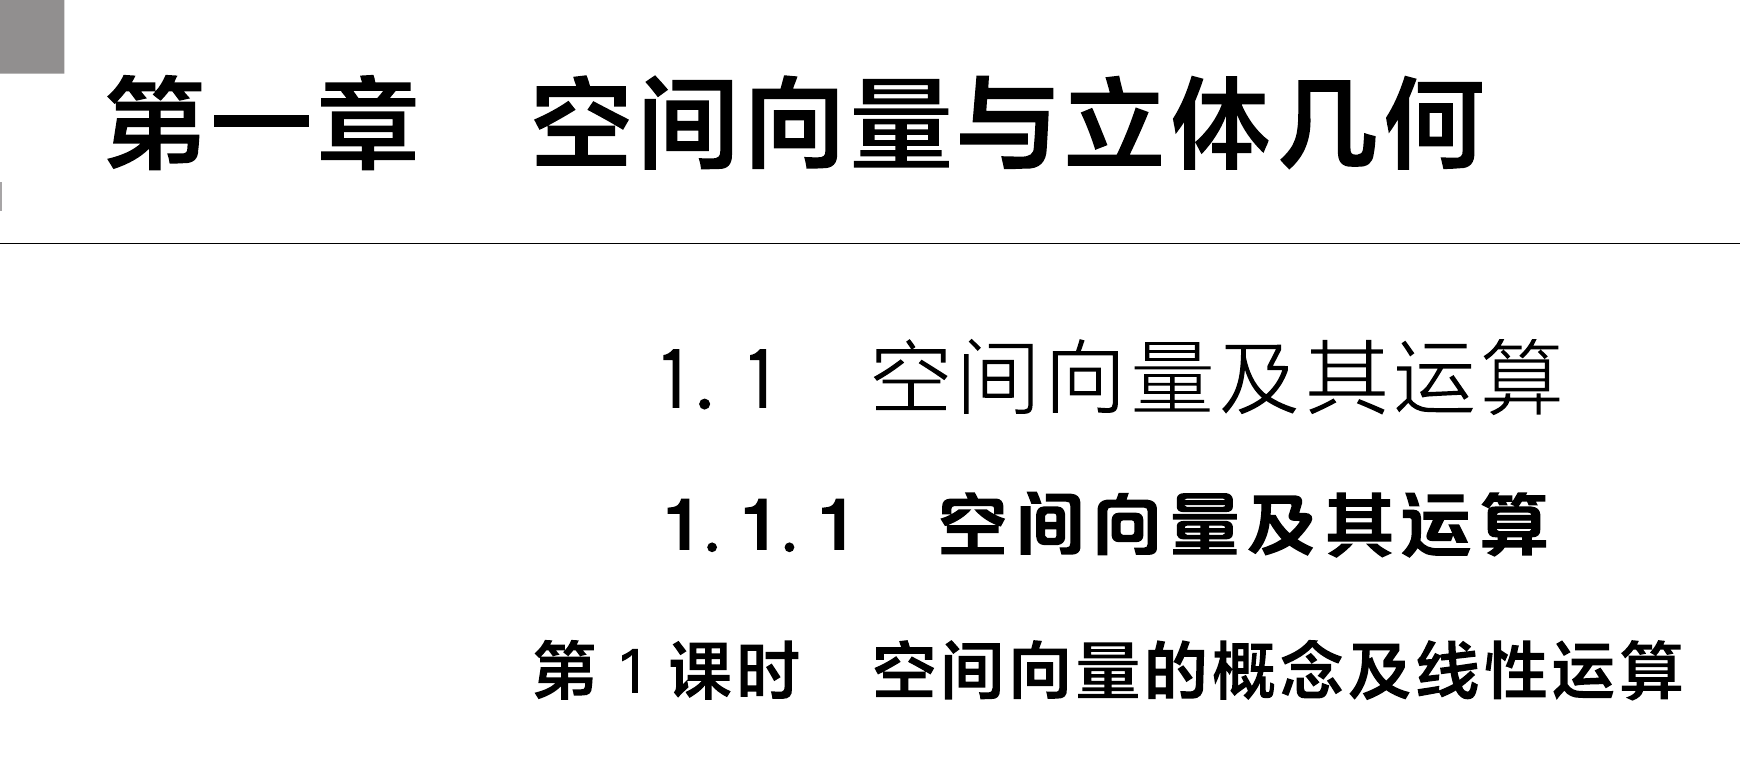
\includegraphics[width=176mm]{qp_章节课时带.png}\par
{\fontsize{8pt}{11pt}\selectfont\color{midgray}↑自上而下：章 20.67pt 级（最重）／节 16.88pt（中粗）／小节 15.1pt／课时 13.0pt（重）。注意全品节标题明显比小节·课时细。}\par
\addvspace{1mm}
\noindent\begin{minipage}[t]{0.52\textwidth}

\includegraphics[width=\linewidth]{qp_知识点一.png}
\par\vspace{0.5mm}{\fontsize{8pt}{11pt}\selectfont\color{midgray}↑p04 ◆知识点一（12pt 级 2.3×）}\par
\end{minipage}\hfill
\begin{minipage}[t]{0.45\textwidth}
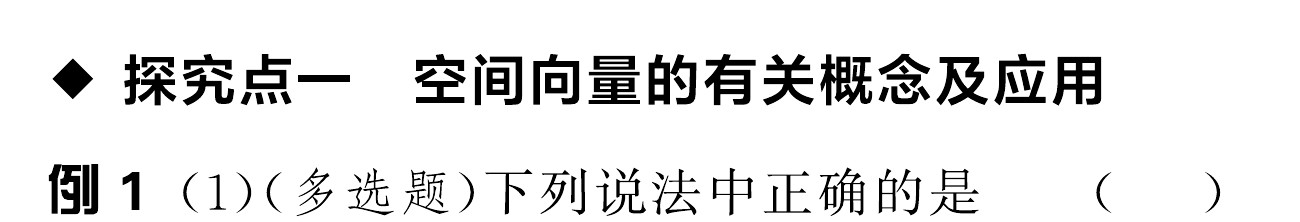
\includegraphics[width=\linewidth]{qp_探究点一例1.png}
\par\vspace{0.5mm}{\fontsize{8pt}{11pt}\selectfont\color{midgray}↑p05 ◆探究点一＋例1 标签（数字为衬线体）}\par
\end{minipage}\par

\candhead{一·思源黑体 Noto Sans SC（Adobe＋Google·SIL OFL 免费商用）}{章=Black 900／节=Medium 500／课时·◆例N=Bold 700／变式=Medium 500}
\lrow{20.67pt}{30pt}{\zhNotoBlk}{\enNotoBlk}{章·Black}{第一章　空间向量与立体几何}
\lrow{16.88pt}{24pt}{\zhNotoMd}{\enNotoMd}{节·Medium}{1.1　空间向量及其运算}
\lrow{13pt}{20pt}{\zhNotoBd}{\enNotoBd}{课时·Bold}{第1课时　空间向量的概念及线性运算}
\lrow{12pt}{17pt}{\zhNotoBd}{\enNotoBd}{◆探究点·例N·Bold}{◆探究点一　空间向量的概念　　例1　(多选题)}
\lrow{12pt}{17pt}{\zhNotoMd}{\enNotoMd}{变式·【】·Medium}{变式1　【学习目标】【诊断分析】}
\lrow{10.5pt}{18pt}{}{}{正文·FZShuSong}{在空间，我们把具有大小和方向的量叫做空间向量．}

\candhead{二·阿里巴巴普惠体（阿里巴巴·官方宣布免费商用，镜像获取）}{章=Heavy／节=Medium／课时·◆例N=Bold／变式=Medium}
\lrow{20.67pt}{30pt}{\zhPuHv}{\enPuHv}{章·Heavy}{第一章　空间向量与立体几何}
\lrow{16.88pt}{24pt}{\zhPuMd}{\enPuMd}{节·Medium}{1.1　空间向量及其运算}
\lrow{13pt}{20pt}{\zhPuBd}{\enPuBd}{课时·Bold}{第1课时　空间向量的概念及线性运算}
\lrow{12pt}{17pt}{\zhPuBd}{\enPuBd}{◆探究点·例N·Bold}{◆探究点一　空间向量的概念　　例1　(多选题)}
\lrow{12pt}{17pt}{\zhPuMd}{\enPuMd}{变式·【】·Medium}{变式1　【学习目标】【诊断分析】}
\lrow{10.5pt}{18pt}{}{}{正文·FZShuSong}{在空间，我们把具有大小和方向的量叫做空间向量．}

\candhead{三·HarmonyOS Sans SC（华为·免费商用）}{章=Black／节=Medium／课时·◆例N=Bold／变式=Medium}
\lrow{20.67pt}{30pt}{\zhHosBlk}{\enHosBlk}{章·Black}{第一章　空间向量与立体几何}
\lrow{16.88pt}{24pt}{\zhHosMd}{\enHosMd}{节·Medium}{1.1　空间向量及其运算}
\lrow{13pt}{20pt}{\zhHosBd}{\enHosBd}{课时·Bold}{第1课时　空间向量的概念及线性运算}
\lrow{12pt}{17pt}{\zhHosBd}{\enHosBd}{◆探究点·例N·Bold}{◆探究点一　空间向量的概念　　例1　(多选题)}
\lrow{12pt}{17pt}{\zhHosMd}{\enHosMd}{变式·【】·Medium}{变式1　【学习目标】【诊断分析】}
\lrow{10.5pt}{18pt}{}{}{正文·FZShuSong}{在空间，我们把具有大小和方向的量叫做空间向量．}

\candhead{四·微软雅黑（本机系统字体）}{{\color{warnred}\bfseries 仅内部参照·不可用于发布（发布权属方正）}}
{\fontsize{9pt}{13pt}\selectfont\color{warnred}\bfseries ▲▲▲ 警示：微软雅黑发布权属方正字库，本页仅作兰亭黑本家形态参照，禁止进入任何发布产物。▲▲▲}\par
\lrow{20.67pt}{30pt}{\zhYhBd}{\enYhBd}{章·Bold（雅黑无更重档）}{第一章　空间向量与立体几何}
\lrow{16.88pt}{24pt}{\zhYhMd}{\enYhMd}{节·Regular}{1.1　空间向量及其运算}
\lrow{13pt}{20pt}{\zhYhBd}{\enYhBd}{课时·Bold}{第1课时　空间向量的概念及线性运算}
\lrow{12pt}{17pt}{\zhYhBd}{\enYhBd}{◆探究点·例N·Bold}{◆探究点一　空间向量的概念　　例1　(多选题)}
\lrow{12pt}{17pt}{\zhYhMd}{\enYhMd}{变式·【】·Regular}{变式1　【学习目标】【诊断分析】}
\lrow{10.5pt}{18pt}{}{}{正文·FZShuSong}{在空间，我们把具有大小和方向的量叫做空间向量．}

\addvspace{4mm}
{\fontsize{16pt}{22pt}\selectfont\bfseries 圆黑标签选美——例N／变式N 标签（12pt 实号＋2×放大）}\par
{\fontsize{8.5pt}{13pt}\selectfont\color{midgray}候选：阿里妈妈方圆体（免费商用，VF 实例化 wght=600/500·BEVL=100 圆角）vs 思源 Medium/Bold。全品裁片同栏对照。}\par
\addvspace{2mm}
\noindent\begin{minipage}[t]{0.24\textwidth}
{\fontsize{8pt}{11pt}\selectfont\color{midgray}方圆体 w600·圆\par}\vspace{0.5mm}
{\fontsize{12pt}{17pt}\selectfont\zhFYa\enFYa 例1\quad 变式1}\par\vspace{1mm}
{\fontsize{24pt}{30pt}\selectfont\zhFYa\enFYa 例1}\par
\end{minipage}\hfill
\begin{minipage}[t]{0.24\textwidth}
{\fontsize{8pt}{11pt}\selectfont\color{midgray}方圆体 w500·圆\par}\vspace{0.5mm}
{\fontsize{12pt}{17pt}\selectfont\zhFYb\enFYb 例1\quad 变式1}\par\vspace{1mm}
{\fontsize{24pt}{30pt}\selectfont\zhFYb\enFYb 例1}\par
\end{minipage}\hfill
\begin{minipage}[t]{0.24\textwidth}
{\fontsize{8pt}{11pt}\selectfont\color{midgray}思源 Medium\par}\vspace{0.5mm}
{\fontsize{12pt}{17pt}\selectfont\zhNotoMd\enNotoMd 例1\quad 变式1}\par\vspace{1mm}
{\fontsize{24pt}{30pt}\selectfont\zhNotoMd\enNotoMd 例1}\par
\end{minipage}\hfill
\begin{minipage}[t]{0.22\textwidth}
{\fontsize{8pt}{11pt}\selectfont\color{midgray}全品真迹（≈2.5×）\par}\vspace{0.5mm}

\includegraphics[width=26mm]{qp_li1_zoom.png}\par
\end{minipage}\par

\end{document}
